\subsection{Generalized fANOVA}
For the classical fANOVA we make the assumption of independent inputs, which is often violated in practice. In the remainder of this section, we therefore investigate what happens, when we allow for dependency between variables. First, let us test with our running example:
\[
h(X_1, X_2) = a + X_1 + 2X_2 + X_1 X_2,
\]

% \subsubsection{fANOVA and the Hoeffding Decomposition}
Now $\rho\neq 0$, while keeping everything else the same. When we follow the exact same logic as above we obtain the following terms:
\begin{align*}
\tilde{y}_{\emptyset} &= \mathbb{E}[g(X_1, X_2)] 
= a + \mathbb{E}[X_1] + 2\mathbb{E}[X_2] + \mathbb{E}[X_1 X_2] \\
&= a + \mathbb{E}[X_1 X_2] 
= a + \left( Cov(X_1, X_2) + \mathbb{E}[X_1]\mathbb{E}[X_2] \right) \\
&= a + \rho \\
\tilde{y}_1(x_1) 
&= \mathbb{E}[g(X_1, X_2) | X_1 = x_1] - \tilde{y}_{\emptyset} \\
&= \mathbb{E}[a + X_1 + 2X_2 + X_1 X_2 | X_1 = x_1] - (a + \rho) \\
&= a + x_1 + 2\mathbb{E}[X_2 | X_1 = x_1] + x_1 \mathbb{E}[X_2 | X_1 = x_1] - a - \rho \\
&= x_1 + \rho(2x_1 + x_1^2 - 1) \\
\tilde{y}_2(x_2) 
&= \mathbb{E}[g(X_1, X_2) \mid X_2 = x_2] - \tilde{y}_{\emptyset} \\
&= \mathbb{E}[a + X_1 + 2X_2 + X_1 X_2 \mid X_2 = x_2] - (a + \rho) \\
&= a + 2x_2 + x_2 \mathbb{E}[X_1 \mid X_2 = x_2] - a - \rho \\
&= 2x_2 + \rho(x_2 + x_2^2 - 1) \\
\tilde{y}_{12}(x_1, x_2) 
&= g(x_1, x_2) - \tilde{y}_{\emptyset} - \tilde{y}_1(x_1) - \tilde{y}_2(x_2) \\
&= a + x_1 + 2x_2 + x_1 x_2 - (a + \rho) - (x_1 + \rho(2x_1 + x_1^2 - 1)) - (2x_2 + \rho(x_2 + x_2^2 - 1))\\
% &= a + x_1 + 2x_2 + x_1 x_2 - (a + \rho) - (x_1 + 2\rho x_1 + \rho x_1^2 - \rho) - (2x_2 + \rho x_2 + \rho x_2^2 - \rho) \\
&= x_1 x_2 - 2\rho x_1 - \rho x_2  - \rho x_1^2  - \rho x_2^2 + \rho
\end{align*}

The fANOVA components are characterized by two central properties zero mean and orthogonality which follow from \autoref{eq:strong_annihilating_conditions}.
When we check if the components $\tilde{y}_0, \tilde{y}_1, \tilde{y}_2, \tilde{y}_{12}$ satisfy these properties, we find out that all components are zero-centred, but not all are orthogonal to each other. We can, for example, immediately see that checking orthogonality between $\tilde{y}_{1}, \tilde{y}_{1,2}$ will yield the expectation over the constant term $\rho$ exactly once, meaning even if all the other expectations cancel out, this constant will remain and the entire expression will be unequal to zero:
\begin{align*}
    \mathbb{E}(\tilde{y}_1(X_1)\tilde{y}_{1,2}(X_1, X_2)) 
    &= \mathbb{E}[(X_1 + 2\rho X_1 + \rho X_1^2 - \rho) \\
    &\quad \cdot (X_1 X_2 - 2\rho X_1 - \rho X_2 - \rho X_1^2 - \rho X_2^2 + \rho)] \\
    &= \mathbb{E}[X_{1}^2X_2] \ldots - \mathbb{E}[\rho^2] \neq 0.
\end{align*}

It turns out that naively computing the ``fANOVA decomposition'' under dependent inputs, results in components that lack orthogonality, which is a crucial property for interpretability.
What we performed in this example is not the fANOVA decomposition for dependent variables but the Hoeffding decomposition \citep{hoeffding1948}.
This shows the need for a more involved approach for a generalization of this method.

\subsubsection{Conditions for Generalized fANOVA}
% \subsection{Generalized fANOVA}
% We base this chapter mainly on the generalization of \cite{rahman2014}, while there exists other work from \cite{hooker2007} or \cite{chastaing2012}. (Write this a bit more detailed: \cite{hooker2007} proofed existence of generalized fANOVA components, proposed estimation scheme, \cite{rahman2014} writes this in more general and measure theoretic fashion and proposes different estimation scheme that he argues is more feasible for high dimensions etc. read more in intro of \cite{rahman2014}; \cite{hooker2007} seems to be viewed as the first one who attempted a generalization to dependent inputs of the entire fANOVA decomposition framework, not just the Sobol indices, and he was inspired by \cite{stone1994}).\par

% As our example illustrated, the classical definition of fANOVA breaks down under dependent inputs.
% Consequently, the terms under dependence have to be defined differently.
\cite{stone1994} inspired the pioneering work of \cite{hooker2007} who offers a first solution to the problem of dependent inputs. Work by \cite{chastaing2012} and \cite{rahman2014} build on his framework with modifications and extensions.\par
% Classical fANOVA boils down to integration w.r.t. the uniform measure and in generalized fANOVA we integrate w.r.t. the distribution of $(X_1, \dots, X_n)$.\par
The generalized fANOVA decomposition still follows the overarching form in \autoref{eq:fanova_decomposition}.
However, we no longer work with a product-type probability measure but now $f_{\boldsymbol{X}}: \mathbb{R} \rightarrow \mathbb{R}_{0}^{+}$ denotes an arbitrary probability density function and $f_{\boldsymbol{X}_u}: \mathbb{R}^u \rightarrow \mathbb{R}_{0}^{+}$ the marginal probability density function of the variables with indices in $u \subseteq d$.\par

Instead of enforcing the strong annihilating conditions for desirable properties of the components, \cite{rahman2014} proposed to formulate a milder version.
The milder version fulfils the same function as the strong annihilating conditions in the classical case but works with the joint density of the variables of interest, instead of the individual marginal probability density functions.
% {\color{red}This makes sense, because when there are dependencies between variables then the individual pdfs would not assign the correct weight to each function value as they ignore the dependence between features in $u$.}
\begin{condition}[Weak annihilating conditions]
    For the generalized fANOVA decomposition we require, that all the non-constant fANOVA terms of variables in $u$ integrate to zero w.r.t. the joint probability density function of variables in $u$:
\begin{equation}
    \int_{\mathbb{R}} y_{u, G}(\boldsymbol{x}_u) f_{\boldsymbol{X}_u}(\boldsymbol{x}_u) d\nu (x_i) = 0 \quad \text{for} \quad i \in u \neq \emptyset
\end{equation}
\end{condition}


% What conditions do they fulfill? Does it differ? Yes, slightly.
If components are defined under the weak annihilating conditions, we can ensure that they have zero mean and satisfy a milder from of orthogonality - hierarchical orthogonality, which means that components of different order are orthogonal to each other while components of the same order are not. Hierarchical orthogonality is the best we can do when independence cannot be assumed.
\begin{proposition}
    % zero mean condition
    Given the weak annihilating conditions, the generalized fANOVA components $y_{u, G}$, with $\emptyset \neq u \subseteq \{1, \ldots, N\}$, are centred around zero:
\begin{equation}
    \mathbb{E}[y_{u, G}(\boldsymbol{X}_u)] := \int_{\mathbb{R}^N} y_{u, G}(\boldsymbol{x}_u) f_{\boldsymbol{X}}(\boldsymbol{x}) \, d\nu (\boldsymbol{x}) = 0.
    \label{eq:zero_mean_g}
\end{equation}
\end{proposition}

\begin{proof}
For any subset $\emptyset \ne u \subseteq \{1, \ldots, N\}$, let $i \in u$. We assume that the weak annihilating conditions hold. Then
\begin{align*}
\mathbb{E}[y_{u,G}(\boldsymbol{X}_u)] 
&:= \int_{\mathbb{R}^N} y_{u,G}(\boldsymbol{x}_u) f_{\boldsymbol{X}}(\boldsymbol{x})\, d \nu (\boldsymbol{x}) \\
&= \int_{\mathbb{R}^{|u|}} y_{u,G}(\boldsymbol{x}_u) \left( \int_{\mathbb{R}^{N - |u|}} f_{\boldsymbol{X}}(\boldsymbol{x}) \, d \nu(\boldsymbol{x}_{-u}) \right) d \nu(\boldsymbol{x}_u) \\
&= \int_{\mathbb{R}^{|u|}} y_{u,G}(\boldsymbol{x}_u) f_u(\boldsymbol{x}_u)\, d \nu(\boldsymbol{x}_u) \\
&= \int_{\mathbb{R}^{|u| - 1}} \left( \int_{\mathbb{R}} y_{u,G}(\boldsymbol{x}_u) f_u(\boldsymbol{x}_u) \, d \nu(\boldsymbol{x}_i) \right) \prod_{j \in u,\, j \ne i} d \nu(\boldsymbol{x}_j) \\
&= 0,
\end{align*}
where we make use of Fubini's theorem and the last line follows from using the weak annihilating condition %~(4.2).
\end{proof}

\begin{proposition}
    % hierarchical orthogonality
    Given the weak annihilating conditions, the fANOVA components are hierarchically orthogonal. This means that for two components $y_{u, G}$ and $y_{v, G}$ with $u \subsetneq v, \emptyset \neq u \subseteq \{1, \ldots, N\}, \emptyset \neq v \subseteq \{1, \ldots, N\} $ it holds that:
\begin{equation}
    \mathbb{E}[y_{u, G}(\boldsymbol{X}_u)y_{v, G}(\boldsymbol{X}_v)] := \int_{\mathbb{R}^N} y_{u, G}(\boldsymbol{x}_u) y_{v, G}(\boldsymbol{x}_v) f_{\boldsymbol{X}}(\boldsymbol{x}) \, d\nu (\boldsymbol{x}) = 0.
\end{equation}
\label{eq:orthogonality_g}
\end{proposition}

\begin{proof}
For any two subsets $\emptyset \ne u \subseteq \{1,\dots,N\}$ and $\emptyset \ne v \subseteq \{1,\dots,N\}$, where $v \subsetneq u$, the subset $u = v \cup (u \setminus v)$. Let $i \in (u \setminus v) \subseteq u$. Then
\begin{align*}
\mathbb{E}[y_{u,G}(\boldsymbol{X}_u) \, y_{v,G}(\boldsymbol{X}_v)]
&:= \int_{\mathbb{R}^N} y_{u,G}(\boldsymbol{x}_u) y_{v,G}(\boldsymbol{x}_v) f_{\boldsymbol{X}}(\boldsymbol{x}) \, d \nu(\boldsymbol{x}) \\
&= \int_{\mathbb{R}^{|u|}} y_{u,G}(\boldsymbol{x}_u) y_{v,G}(\boldsymbol{x}_v) \left( \int_{\mathbb{R}^{N - |u|}} f_{\boldsymbol{X}}(\boldsymbol{x}) \, d \nu(\boldsymbol{x}_{-u}) \right) d \nu(\boldsymbol{x}_u) \\
&= \int_{\mathbb{R}^{|u|}} y_{u,G}(\boldsymbol{x}_u) y_{v,G}(\boldsymbol{x}_v) f_u(\boldsymbol{x}_u) \, d \nu(\boldsymbol{x}_u) \\
&= \int_{\mathbb{R}^{|v|}} y_{v,G}(\boldsymbol{x}_v)
    \int_{\mathbb{R}^{|u \setminus v|}} y_{u,G}(\boldsymbol{x}_u) f_u(\boldsymbol{x}_u) \, d \nu(\boldsymbol{x}_{u \setminus v}) \, d \nu(\boldsymbol{x}_v) \\
&= \int_{\mathbb{R}^{|v|}} y_{v,G}(\boldsymbol{x}_v)
    \int_{\mathbb{R}^{|u \setminus v| - 1}} \left( \int_{\mathbb{R}} y_{u,G}(\boldsymbol{x}_u) f_u(\boldsymbol{x}_u) \, d \nu(\boldsymbol{x}_i) \right)
    \prod_{\substack{j \in (u \setminus v) \\ j \ne i}} d \nu(\boldsymbol{x}_j) \, d \nu(\boldsymbol{x}_v) \\
&= 0.
\end{align*}
Repeatedly using Fubini's theorem and the weak annihilating conditions the equality to zero follows.
\end{proof}

A key contribution from \cite{hooker2007} and \cite{rahman2014} is that they construct a generalization of the fANOVA decomposition method as a whole, not only parts, such as the Sobol indices.
This means it is important that Rahman's generalized statements are coherent with the classical fANOVA decomposition.
\begin{proposition}
    The weak annihilating conditions become the strong annihilating conditions under independence assumption.
    \label{prop:weak_strong}
\end{proposition}

\begin{proof}
Assume that the random variables $\{X_j\}_{j \in u}$ are independent. Then we can factorize the marginal density $f_u(\boldsymbol{x}_u)$ as
\[
f_u(\boldsymbol{x}_u) = \prod_{j \in u} f_{X_j}(x_j).
\]
Now consider the weak annihilating condition~(4.2) for some $i \in u \neq \emptyset$:
\[
\int_{\mathbb{R}} y_{u,G}(\boldsymbol{x}_u) f_u(\boldsymbol{x}_u) \, d \nu(\boldsymbol{x}_i) = 0.
\]
Since we assume independence, we can substitute the joint marginal density with the product of the marginal densities:
\[
\int_{\mathbb{R}} y_{u,G}(\boldsymbol{x}_u) \left( \prod_{j \in u} f_{X_j}(x_j) \right) d \nu(\boldsymbol{x}_i) = 0.
\]
For fixed $x_j$ with $j \ne i$, the terms $f_{X_j}(x_j)$ are constant with respect to $x_i$, and can therefore be pulled out of the integral:
\[
\left( \prod_{j \in u,\, j \ne i} f_{X_j}(x_j) \right) \int_{\mathbb{R}} y_{u,G}(\boldsymbol{x}_u) f_{X_i}(x_i) \, d \nu(x_i) = 0.
\]
As product of probability density functions the prefactor is strictly positive for all $x_j$ with $j \ne i$. Therefore, the integral must be zero for the equality to hold:
\[
\int_{\mathbb{R}} y_{u,G}(\boldsymbol{x}_u) f_{X_i}(x_i) \, d \nu(x_i) = 0,
\]
which are the strong annihilating conditions \autoref{eq:strong_annihilating_conditions}.
\end{proof}


\subsubsection{Construction of the Generalized fANOVA Terms}
Recall the construction of the classical fANOVA components \autoref{eq:fanova_components_classical}. The equation tells us that the non-constant classical fANOVA components are defined via the integral of the original function w.r.t. to the product-type probability density function, minus effects by other terms. So ideally for a well-aligned generalization, we would want that the general fANOVA terms can be understood in a similar way, as the integral of $y$ w.r.t. \textit{a smartly chosen} probability density function, minus effects explained by other terms.
This is exactly what \cite{rahman2014} accomplishes.
To understand this, we first need to distinguish three cases of integration that will occure in the construction of the generalized components.

% Following a similar logic as for the classical fANOVA decomposition, one can integrate the desired decomposition w.r.t. to a suitable pdf and set the (weak) annihilating conditions to obtain the fANOVA decomposition. They key is to find this suitable pdf which results in the desired integral. \cite{rahman2014} proposes $f_{-u}(\boldsymbol{x}_{-u})$. In Theorem 4.4. he shows how the generalized fANOVA components constructed by this look like. And Lemma 4.3 is a helping statement, that should cover all the integral cases that appear in Theorem 4.4. and allow us to write the expressions in Theorem 4.4. in the reduced form we see them.

\begin{proposition}\label{prop:integration_cases}
Consider the generalized fANOVA components $y_{v,G}$, $\emptyset \ne v \subseteq \{1,\dots,N\}$, of a square-integrable function $y : \mathbb{R}^N \to \mathbb{R}$. When integrated w.r.t. the probability measure $f_{-u}(\boldsymbol{x}_{-u})\, d \nu(\boldsymbol{x}_{-u})$, $u \subseteq \{1,\dots,N\}$, one can distinguish three cases:
\begin{equation}
\begin{aligned}
& \int_{\mathbb{R}^{N - |u|}} y_{v,G}(\boldsymbol{x}_v) 
    f_{-u}(\boldsymbol{x}_{-u}) \, d \nu(\boldsymbol{x}_{-u}) \\[0.5em]
&= 
\begin{cases}
    \displaystyle 
    \int_{\mathbb{R}^{|v \cap -u|}} 
        y_{v,G}(\boldsymbol{x}_v)\,
        f_{v \cap -u}(\boldsymbol{x}_{v \cap -u})\,
        d \nu(\boldsymbol{x}_{v \cap -u}) 
        & \text{if } v \cap u \ne \emptyset \text{ and } v \not\subset u, \\[1ex]
    y_{v,G}(\boldsymbol{x}_v) 
        & \text{if } v \cap u \ne \emptyset \text{ and } v \subseteq u, \\[1ex]
    0 
        & \text{if } v \cap u = \emptyset.
\end{cases}
\end{aligned}
\end{equation}
\label{prop:integration_cases}
\end{proposition}

\begin{proof}
Let $u \subseteq \{1,\dots,N\}$ and $\emptyset \ne v \subseteq \{1,\dots,N\}$. We distinguish between three types of relationships between $v$ and $u$.

Before analysing the first case, note that for any such $u$ and $v$, it is possible to write
\[
(v \cap -u) \subseteq -u \quad \text{and} \quad -u = (-u \setminus (v \cap -u)) \cup (v \cap -u),
\]
which will be used in the integral decomposition below.

\paragraph{Case 1: \( v \cap u \ne \emptyset \) and \( v \not\subseteq u \)}
We use the decomposition of $-u$ stated above to decompose the integration over $\boldsymbol{x}_{-u}$ as:

\begin{equation}
\begin{aligned}
&\int_{\mathbb{R}^{N - |u|}} 
    y_{v,G}(\boldsymbol{x}_v)\,
    f_{-u}(\boldsymbol{x}_{-u}) 
    \, d \nu(\boldsymbol{x}_{-u}) \\[0.5em]
&= \int_{\mathbb{R}^{|v \cap -u|}} 
    y_{v,G}(\boldsymbol{x}_v)
    \left(
        \int_{\mathbb{R}^{N - |u| - |v \cap -u|}}
            f_{-u}(\boldsymbol{x}_{-u \setminus (v \cap -u)}, \boldsymbol{x}_{v \cap -u})
            \, d \nu(\boldsymbol{x}_{-u \setminus (v \cap -u)})
    \right) 
    d \nu(\boldsymbol{x}_{v \cap -u}) \\
    &= \int_{\mathbb{R}^{|v \cap -u|}} y_{v,G}(\boldsymbol{x}_v) f_{v \cap -u}(\boldsymbol{x}_{v \cap -u}) \, d\boldsymbol{x}_{v \cap -u},
\end{aligned}
\end{equation}
where the inner integral integrates out all variables in 
$-u \setminus (v \cap -u)$, 
resulting in the marginal density 
$f_{v \cap -u}(\boldsymbol{x}_{v \cap -u})$.

\begin{center}
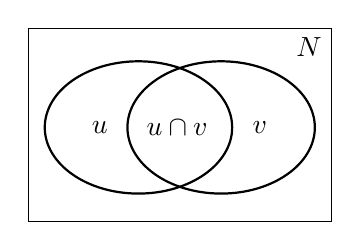
\begin{tikzpicture}[scale=0.7]
  % Rectangle representing N (lighter, not focus)
  \draw[black, thin, opacity=1] (-1.5,-1.5) rectangle (4,2) 
        node[anchor=north east] {$\mathbb{N}$};

  % Set u (ellipse)
  \draw[thick] (0.5,0.2) ellipse (1.7cm and 1.2cm);
  \node at (-0.2,0.2) {$u$};

  % Set v (ellipse)
  \draw[thick] (2.0,0.2) ellipse (1.7cm and 1.2cm);
  \node at (2.7,0.2) {$v$};

  % Intersection label
  \node at (1.2,0.2) {$u \cap v$};
\end{tikzpicture}
\end{center}

\paragraph{Case 2: $v \cap u \ne \emptyset \text{ and } v \subseteq u$.}
Since the sets $v$ and $-u$ are then completely disjoint, $y_{v,G}(\boldsymbol{x}_v)$ is independent of $\boldsymbol{x}_{-u}$ and can be pulled out of the integral:
\[
\int_{\mathbb{R}^{N - |u|}} y_{v,G}(\boldsymbol{x}_v) f_{-u}(\boldsymbol{x}_{-u}) \, d \nu(\boldsymbol{x}_{-u})
= y_{v,G}(\boldsymbol{x}_v) \int_{\mathbb{R}^{N - |u|}} f_{-u}(\boldsymbol{x}_{-u}) \, d \nu(\boldsymbol{x}_{-u})
= y_{v,G}(\boldsymbol{x}_v),
\]
which works because $f_{-u}$ integrates to one.

\begin{center}
    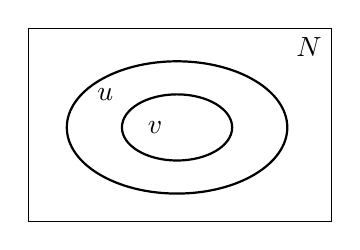
\begin{tikzpicture}[scale=0.7]
  % Rectangle for N (light, not focus)
  \draw[black, thin, opacity=1] (-1.5,-1.5) rectangle (4,2) 
        node[anchor=north east] {$\mathbb{N}$};

  % Set u (outer ellipse)
  \draw[thick] (1.2,0.2) ellipse (2.0cm and 1.2cm);
  \node at (-0.1,0.8) {$u$};

  % Set v (nested inside)
  \draw[thick] (1.2,0.2) ellipse (1.0cm and 0.6cm);
  \node at (0.8,0.2) {$v$};
\end{tikzpicture}
\end{center}

\paragraph{Case 3: \( v \cap u = \emptyset \).}
In this case, we have \( v \subseteq -u \), so \( v \cap -u = v \). Then we can write:
\[
\begin{aligned}
\int_{\mathbb{R}^{N - |u|}} y_{v,G}(\boldsymbol{x}_v) f_{-u}(\boldsymbol{x}_{-u}) \, d \nu(\boldsymbol{x}_{-u})
&= \int_{\mathbb{R}^{|v|}} y_{v,G}(\boldsymbol{x}_v)
\left( \int_{\mathbb{R}^{N - |u| - |v|}} f_{-u}(\boldsymbol{x}_{-u}) \, d \nu(\boldsymbol{x}_{-u \setminus v}) \right)
d \nu(\boldsymbol{x}_v) \\
&= \int_{\mathbb{R}^{|v|}} y_{v,G}(\boldsymbol{x}_v) f_v(\boldsymbol{x}_v) \, d \nu(\boldsymbol{x}_v) \\
&= \int_{\mathbb{R}^{|v|-1}} \left( \int_{\mathbb{R}} y_{v,G}(\boldsymbol{x}_v) f_v(\boldsymbol{x}_v) \, d \nu(x_i) \right)
\prod_{\substack{j \in v \\ j \ne i}} d \nu (x_j) \\
&= 0,
\end{aligned}
\]
while we again split the interval in such a way that we recognize the marginal density $f_v$ and make use of the zero mean property from the strong annihilating conditions.
\begin{center}
    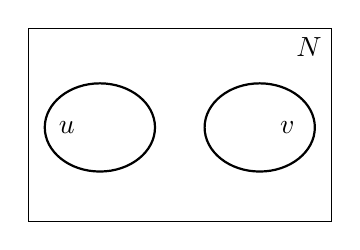
\begin{tikzpicture}[scale=0.7]
  % Rectangle for N (lighter, not focus)
  \draw[black, thin, opacity=1] (-1.5,-1.5) rectangle (4,2)
        node[anchor=north east] {$\mathbb{N}$};

  % Set u (left, ellipse)
  \draw[thick] (-0.2,0.2) ellipse (1cm and 0.8cm);
  \node at (-0.8,0.2) {$u$};

  % Set v (right, ellipse, disjoint from u)
  \draw[thick] (2.7,0.2) ellipse (1cm and 0.8cm);
  \node at (3.2,0.2) {$v$};

  % Example index i inside v (optional)
  % \node at (2.5,-0.2) {$i$};
\end{tikzpicture}
\end{center}

\end{proof}

As we will see in the following, we will encounter all of these three integration cases in the definition of the generalized fANOVA components à la \cite{rahman2014}.
In \autoref{prop:integration_cases} we also already see that the smartly chosen probability density function is $f_{-u}(\boldsymbol{x}_{-u})$.


\begin{proposition}
The generalized fANOVA component functions \( y_{u,G}(\boldsymbol{x}_u), u \subseteq \{1,\dots,N\} \) of a square-integrable function $y:\mathbb{R}^N \to \mathbb{R}$ for a given probability measure $f_{\boldsymbol{X}} d\nu(\boldsymbol{x})$ of $\boldsymbol{X} \in \mathbb{R}^N$ can be recursively defined via the following set of equations:
\begin{align}
y_{\emptyset,G} &= \int_{\mathbb{R}^N} y(\boldsymbol{x}) f_{\boldsymbol{X}}(\boldsymbol{x}) \, d \nu(\boldsymbol{x}) \\
y_{u,G}(\boldsymbol{X}_u) &= \int_{\mathbb{R}^{N - |u|}} y(\boldsymbol{X}_u, \boldsymbol{x}_{-u}) f_{-u}(\boldsymbol{x}_{-u}) \, d \nu(\boldsymbol{x}_{-u})
- \sum_{v \subsetneq u} y_{v,G}(\boldsymbol{X}_v) \notag \\
&\quad - \sum_{\substack{\emptyset \ne v \subseteq \{1,\dots,N\} \\ v \cap u \ne \emptyset,\ v \not\subset u}} 
\int_{\mathbb{R}^{|v \cap -u|}} y_{v,G}(\boldsymbol{X}_{v \cap u}, \boldsymbol{x}_{v \cap -u}) f_{v \cap -u}(\boldsymbol{x}_{v \cap -u}) \, d \nu(\boldsymbol{x}_{v \cap -u}).
\end{align}
\label{prop:generalized_fanova_components_rahman}
\end{proposition}


\begin{proof}
We begin by integrating both sides of the generalized fANOVA decomposition
\[
y(\boldsymbol{x}) = \sum_{v \subseteq \{1,\dots,N\}} y_{v,G}(\boldsymbol{x}_v)
\]
w.r.t. $f_{-u}(\boldsymbol{x}_{-u})\, d \nu(\boldsymbol{x}_{-u})$, replacing $\boldsymbol{X}$ by $\boldsymbol{x}$, and changing the dummy index from $u$ to $v$. This yields:
\[
\int_{\mathbb{R}^{N - |u|}} y(\boldsymbol{x}) f_{-u}(\boldsymbol{x}_{-u}) \, d \nu(\boldsymbol{x}_{-u})
= \sum_{v \subseteq \{1,\dots,N\}} \int_{\mathbb{R}^{N - |u|}} y_{v,G}(\boldsymbol{x}_v) f_{-u}(\boldsymbol{x}_{-u}) \, d \nu(\boldsymbol{x}_{-u}).
\]

\paragraph{Case: \( u = \emptyset \).}
We set $u = \emptyset$, so $-u = \{1,\dots,N\}$ and $f_{-u}(\boldsymbol{x}_{-u}) d \nu(\boldsymbol{x}_{-u}) = f_{\boldsymbol{X}}(\boldsymbol{x}) d \nu(\boldsymbol{x})$. The above integral can then be written as:
\[
\int_{\mathbb{R}^N} y(\boldsymbol{x}) f_{\boldsymbol{X}}(\boldsymbol{x}) \, d \nu(\boldsymbol{x})
= \sum_{v \subseteq \{1,\dots,N\}} \int_{\mathbb{R}^N} y_{v,G}(\boldsymbol{x}_v) f_{\boldsymbol{X}}(\boldsymbol{x}) \, d \nu(\boldsymbol{x})
\]
\[
= y_{\emptyset,G}
+ \sum_{\emptyset \ne v \subseteq \{1,\dots,N\}} \int_{\mathbb{R}^N} y_{v,G}(\boldsymbol{x}_v) f_{\boldsymbol{X}}(\boldsymbol{x}) \, d \nu(\boldsymbol{x})
\]
\[
= y_{\emptyset,G} + \sum_{\emptyset \ne v \subseteq \{1,\dots,N\}} \mathbb{E}[y_{v,G}(\boldsymbol{X}_v)] = y_{\emptyset,G},
\]
where the last sum vanishes under the weak annihilating condition.

\paragraph{Case: \( \emptyset \ne u \subseteq \{1,\dots,N\} \).}
We return to the integrated decomposition
\[
\int_{\mathbb{R}^{N - |u|}} y(\boldsymbol{x}) f_{-u}(\boldsymbol{x}_{-u}) \, d\boldsymbol{x}_{-u}
= \sum_{v \subseteq \{1,\dots,N\}} \int_{\mathbb{R}^{N - |u|}} y_{v,G}(\boldsymbol{x}_v) f_{-u}(\boldsymbol{x}_{-u}) \, d\boldsymbol{x}_{-u},
\]
and apply \autoref{prop:integration_cases} to evaluate each term in the sum according to the relationship between $v$ and $u$:

\begin{itemize}
  \item[\textbf{(A)}] \( v \cap u \ne \emptyset \) and \( v \not\subset u \): \\
  This is case 1 of \autoref{prop:integration_cases}. The integral becomes:
  \[
  \sum_{\substack{\emptyset \ne v \subseteq \{1,\dots,N\} \\ v \cap u \ne \emptyset,\ v \not\subset u}} 
  \int_{\mathbb{R}^{|v \cap -u|}} y_{v,G}(\boldsymbol{x}_v) f_{v \cap -u}(\boldsymbol{x}_{v \cap -u}) \, d\boldsymbol{x}_{v \cap -u}.
  \]

  \item[\textbf{(B)}] \( v \subsetneq u \): \\
  This is contained in case 2 of \autoref{prop:integration_cases}. The integrals reduce to the component functions themselves:
  \[
  \sum_{v \subsetneq u} y_{v,G}(\boldsymbol{x}_v).
  \]

  \item[\textbf{(C)}] \( v = u \): \\
  This is also contained in case 2 of \autoref{prop:integration_cases}. The integral becomes:
  \[
  y_{u,G}(\boldsymbol{x}_u).
  \]

  \item[\textbf{(D)}] \( v \cap u = \emptyset \): \\
  This is case 3 of \autoref{prop:integration_cases}. These terms vanish:
  \[
  \sum_{\substack{v \subseteq \{1,\dots,N\} \\ v \cap u = \emptyset}} 0 = 0.
  \]
\end{itemize}

Putting everything together:
\[
\begin{aligned}
&\int_{\mathbb{R}^{N - |u|}} y(\boldsymbol{x}) f_{-u}(\boldsymbol{x}_{-u}) 
    \, d\boldsymbol{x}_{-u} \\
&= y_{u,G}(\boldsymbol{x}_u)
   + \sum_{v \subsetneq u} y_{v,G}(\boldsymbol{x}_v) + 
   \sum_{\substack{\emptyset \ne v \subseteq \{1,\dots,N\} \\
                   v \cap u \ne \emptyset,\ v \not\subset u}} 
   \int_{\mathbb{R}^{|v \cap -u|}} 
        y_{v,G}(\boldsymbol{x}_v) 
        f_{v \cap -u}(\boldsymbol{x}_{v \cap -u}) 
        \, d\boldsymbol{x}_{v \cap -u}.
\end{aligned}
\]


Rearranging gives the almost final expression for \( y_{u,G}(\boldsymbol{x}_u) \):
\[
\begin{aligned}
&y_{u,G}(\boldsymbol{x}_u) \\
&= \int_{\mathbb{R}^{N - |u|}} y(\boldsymbol{x}) f_{-u}(\boldsymbol{x}_{-u}) \, d\boldsymbol{x}_{-u}
- \sum_{v \subsetneq u} y_{v,G}(\boldsymbol{x}_v)
- \sum_{\substack{\emptyset \ne v \subseteq \{1,\dots,N\} \\ v \cap u \ne \emptyset,\ v \not\subset u}} 
\int_{\mathbb{R}^{|v \cap -u|}} y_{v,G}(\boldsymbol{x}_v) f_{v \cap -u}(\boldsymbol{x}_{v \cap -u}) \, d\boldsymbol{x}_{v \cap -u}.
\end{aligned}
\]
As a final step, we only have to write \( v = (v \cap u) \cup (v \cap -u) \) to obtain the expression of \autoref{prop:generalized_fanova_components_rahman}.

\end{proof}

% Alternative definition of components by Hooker
\subsubsection{Generalization via Projection}
\cite{hooker2007} approaches his generalization of the fANOVA decomposition from the angle of orthogonal projections. Instead of the more recursive definition of the components functions as in \cite{rahman2014}, he defines the fANOVA components as a joint set which simultaneously minimizes the squared difference to the original function $y$ under certain constraints.
The constraints he sets for the optimization problem should ensure that the generalized components satisfy the desired properties of zero mean and hierarchical orthogonality.

The generalized fANOVA terms $\{y_u(x_u) | u \subseteq d \}$ jointly satisfiy:
\begin{equation}
\left\{ y_{u, G}(\boldsymbol{x}_u) \,\middle|\, u \subseteq d \right\}
= \arg\min_{\{g_u \in \mathcal{L}^2(\mathbb{R}^{|u|})\}} 
\int_{\mathbb{R}^N} \left( \sum_{u \subseteq d} g_u(\boldsymbol{x}_u) - y(\boldsymbol{x}) \right)^2 f_{\boldsymbol{X}}(\boldsymbol{x}) \, d \nu (\boldsymbol{x})
\label{prop:generalized_fanova_components_hooker}
\end{equation}
under the hierarchical orthogonality conditions:
\begin{equation}
    \forall v \subseteq u,\ \forall g_v : \int_{\mathbb{R}^N} y_u(\boldsymbol{x}_u) g_v(\boldsymbol{x}_v) f_{\boldsymbol{X}}(\boldsymbol{x}) \, d \nu (\boldsymbol{x}) = 0.
\label{eq:hooker_hierarchical_orthogonality}
\end{equation}

In Hookers definition we recognize a projection. We are simultaneously finding the set of components functions $g_u$ that minimize the weighted squared difference to the original function $y$ (under the given integral constraint), which is exactly the definition of a projection of $y$ onto a specific subspace $\mathcal{G}$.\par

However, the constraint in \autoref{eq:hooker_hierarchical_orthogonality} is infeasible to enforce in practice. 
Therefore, Hooker formulated the following proposition, which ensures hierarchical orthogonality of the fANOVA components and thus forms the building block of his approach. It can be compared to the weak annihilating conditions in \cite{rahman2014}.
\begin{proposition}
    The hierarchical orthogonality of the fANOVA components is ensured if and only if the following integral condition holds:
    \begin{equation}
\forall u \subseteq N,\ \forall i \in u:\ \int_{\mathbb{R}^N} y_u(\boldsymbol{x}_u) f_{\boldsymbol{X}}(\boldsymbol{x})\, d \nu (x_i)\, d \nu (\boldsymbol{x}_{-u}) = 0.
\end{equation}
\label{prop:hooker_hierarchical_orthogonality}
\end{proposition}

\begin{proof}
    The proof is organized in two parts. First, Hooker showed that, the hierarchical orthogonality is true, if the integral conditions hold. Second he shows that hierarchical orthogonality breaks down if the integral conditions are not true.\par
    For the first part, assume that \autoref{prop:hooker_hierarchical_orthogonality} holds. Let $i \in u \setminus v$, then $y_v(\boldsymbol{x}_v)$ is independent of $x_i$ and $\boldsymbol{x}_{-u}$, so we can write:
\begin{equation}
\begin{aligned}
\langle y_u, y_v \rangle 
&:= \int_{\mathbb{R}^N} 
        y_v(\boldsymbol{x}_v)\, y_u(\boldsymbol{x}_u)\, 
        f_{\boldsymbol{X}}(\boldsymbol{x})\, 
        d \nu(\boldsymbol{x}) \\[0.3em]
&= y_v(\boldsymbol{x}_v) 
   \int_{\mathbb{R}^N} 
        y_u(\boldsymbol{x}_u)\, 
        f_{\boldsymbol{X}}(\boldsymbol{x})\, 
        d \nu(\boldsymbol{x}) \\[0.3em]
&= 0.
\end{aligned}
\end{equation}

For the second part, assume that there exists a subset $u$ and an index $i$ for which \autoref{prop:hooker_hierarchical_orthogonality} does not hold, i.e.
    \begin{equation}
        \int_{\mathbb{R}^N} y_u(\boldsymbol{x}_u)\, f_{\boldsymbol{X}}(\boldsymbol{x})\, d \nu (x_i)\, d \nu (x_{-u}) \ne 0 \quad \text{for some} \quad i, u.
    \end{equation}
    Further, assume that \autoref{prop:hooker_hierarchical_orthogonality} holds for all subsets $v \neq u$ and indices $j \neq i$. Hooker then constructs a fANOVA term $y_v$ with lower order than $y_u$, which is not orthogonal to $y_u$. He sets $v = u \setminus \{i\}$, so $y_v$ is one order lower than $y_u$ and defined as:
    \begin{equation}
        y_v(\boldsymbol{x}_v) := \int_{\mathbb{R}^N} f_u(\boldsymbol{x}_u) \, f_{\boldsymbol{X}}(\boldsymbol{x}) \, d \nu (x_i) \, d \nu (\boldsymbol{x}_{-u}).
    \end{equation}
    $y_v$ is a valid fANOVA component, which is unequal to zero by assumption of \autoref{prop:hooker_hierarchical_orthogonality} being false, while it itself satisfies \autoref{prop:hooker_hierarchical_orthogonality} by assumption:
    \begin{equation}
        \forall j \in v, \quad \int_{\mathbb{R}^N} y_v(\boldsymbol{x}_v) \, f_{\boldsymbol{X}}(\boldsymbol{x}) \, d \nu (x_j) \, d \nu (\boldsymbol{x}_{-v}) = 0.
    \end{equation}
 Hooker then shows that $y_v$ is not orthogonal to $y_u$:
\begin{equation}
    \begin{aligned}
        \langle y_u, y_v \rangle
        &= \int_{\mathbb{R}^N} y_u(\boldsymbol{x}_u) \, y_v(\boldsymbol{x}_v) \, f_X(\boldsymbol{x}) \, d \nu(\boldsymbol{x}) \\
        &= \int_{\mathbb{R}^N} y_u(\boldsymbol{x}_u) \left( \int_{\mathbb{R}^N} y_u(\boldsymbol{x}_u) \, f_X(\boldsymbol{x}) \, d \nu(x_i) \, d \nu(\boldsymbol{x}_{-u}) \right) f_{\boldsymbol{X}}(\boldsymbol{x}) \, d \nu(\boldsymbol{x}) \\
        &= \int_{\mathbb{R}^N} \left( \int_{\mathbb{R}^N} y_u(\boldsymbol{x}_u) \, f_X(\boldsymbol{x}) \, d \nu(x_i) \, d \nu(\boldsymbol{x}_{-u}) \right)^2 d \nu(\boldsymbol{x}_{u \setminus \{i\}}) \\
        &\neq 0.
    \end{aligned}
\end{equation}

\end{proof}


Hooker approaches his generalization through the lense of projections while Rahman gives a form that tries to imitate the classical fANOVA terms. A crucial paralel of both versions which dinstiguishes them from the classical case is that their components are defined in dependence of each other (\autoref{prop:generalized_fanova_components_rahman}, \autoref{prop:generalized_fanova_components_hooker}).
% In the Rahman approach, the components are derived from the original function by integrating out the other variables, while in the Hooker approach, the components are defined through a minimization problem that seeks to best approximate the original function.
This makes it in general difficult to compute the generalized fANOVA components analytically, even for simple functions.


\subsubsection{Generalized Variance Decomposition}
Given that the fANOVA decomposition changes under dependent inputs, we briefly make an adjustment to the second-moment statistics of the generalized fANOVA decomposition.
The mean of $y$ remains unchanged and is still given by the constant term \( y_{\emptyset,G} \), i.e.
\[
\mu_G := \mathbb{E}[y(\boldsymbol{X})] = y_{\emptyset,G}.
\]

In contrast, the variance decomposition looks different, as cross-terms of the same order do not vanish under hierarchical orthogonality.
For $ \emptyset \neq u \subseteq \{1,\dots,N\}$, $\emptyset \neq v \subseteq \{1,\dots,N\}$, $u \neq v$ we restate from above:
\begin{align}
\sigma^2 
&:= \mathbb{E}\left[ \left( y(\boldsymbol{X}) - \mu_G \right)^2 \right] \notag \\
&= \mathbb{E} \left[ \left( y_{\emptyset,G} + \sum_{u} y_{u,G}(\boldsymbol{X}_u) - y_{\emptyset,G} \right)^2 \right] \notag \\
&= \mathbb{E} \left[ \left( \sum_{u} y_{u,G}(\boldsymbol{X}_u) \right)^2 \right] \notag \\
&= \sum_{u} \mathbb{E} \left[ y_{u,G}^2(\boldsymbol{X}_u) \right]
+ \sum_{\substack{u \not\subseteq v,\, v \not\subseteq u}} 
\mathbb{E} \left[ y_{u,G}(\boldsymbol{X}_u) y_{v,G}(\boldsymbol{X}_v) \right],
\end{align}
while the first sum in the final line goes over all nonempty subsets $u$ and the second sum goes over all pairs of subsets $(u, v)$ where neither is a subset of the other one.
Conceptually this means that the first term is the sum of the variances of the components, while the second term is the sum of the covariances between components that are not hierarchically orthogonal.
The indices under the second component capture precisely the cross-terms that do not vanish under hierarchical orthogonality. As we saw earlier, cross-terms of the same hierarchy also cancel out under the orthogonality assumption of the classical fANOVA.



\subsubsection{Example: Dependent Multivariate Normal Inputs}
For the end of this section, it remains to answer how the true generalized fANOVA decomposition looks like for our running example.
While the interdependence of the generalized components makes it difficult to arrive at an analytical solution, \cite{rahman2014} provides a way to obtain the closed-from solution for any polynomial of maximum two degree under normally distributed input variables.\par

The idea in \cite{rahman2014} is based on Fourier-Polynomial expansion, which allows to write each generalized fANOVA component as a weighted sum of basis functions. 
The problem shifts from finding the fANOVA component functions to finding the basis functions which allow us to express the fANOVA terms.
Rahman chooses Hermite polynomials as basis functions, which are by construction zero mean and hierarchical orthogonal. Satisfying these properties, the Hermite polynomial basis functions ensure fANOVA components that are also zero mean and hierarchical orthogonal.
The challenge that remains is to find the weights for the basis functions, which can be done via coefficient matching; at least for a polynomial of degree two.

% The idea
A polynomial of degree two has the general form
$$y(x_1,x_2) = a_0 + a_1 x_1 + a_2 x_2 + a_{11} x_1^2 + a_{22} x_2^2 + a_{12} x_1 x_2.$$
We know that any such polynomial may be expressed as a sum of weighted basis functions \cite{nagler2024linalg} of the form:

\begin{align*}
y(x_1,x_2) 
&= c_0 
  + c_{1,1}\,\psi_{1,1}(x_1) 
  + c_{2,1}\,\psi_{2,1}(x_2)
  + c_{1,2}\,\psi_{1,2}(x_1)
  + c_{2,2}\,\psi_{2,2}(x_2)
  + c_{12, 11}\,\psi_{12, 11}(x_1,x_2),
\end{align*}
where the $\psi_{i,j}$ are the basis functions with corresponding weights $c_0, \dots , c_{12, 11} \in \mathbb{R}$.

The idea is to carefully construct a set of basis functions which fulfill zero mean 
and hierarchical orthogonality. Then the expansion in these basis functions is already the 
fANOVA decomposition of a quadratic polynomial, i.e.
\begin{align*}
y(x_1,x_2) 
&= a_0 + a_1 x_1 + a_2 x_2 + a_{11} x_1^2 + a_{22} x_2^2 + a_{12} x_1 x_2 \\[3pt]
&= c_0 
  + c_{1,1}\,\psi_{1,1}(x_1) 
  + c_{2,1}\,\psi_{2,1}(x_2)
  + c_{1,2}\,\psi_{1,2}(x_1)
  + c_{2,2}\,\psi_{2,2}(x_2)
  + c_{12, 11}\,\psi_{12, 11}(x_1,x_2) \\[3pt]
&= 
\underbrace{c_0}_{y_0}
+ \underbrace{\big(c_{1,1}\,\psi_{1,1}(x_1) 
                + c_{1,2}\,\psi_{1,2}(x_1)\big)}_{y_1(x_1)}
+ \underbrace{\big(c_{2,1}\,\psi_{2,1}(x_2) 
                + c_{2,2}\,\psi_{2,2}(x_2)\big)}_{y_2(x_2)}
+ \underbrace{c_{12, 11}\,\psi_{12, 11}(x_1,x_2)}_{y_{12}(x_1,x_2)}.
\end{align*}


Derived from the probability density of a multivariate normal distribution, \cite{rahman2014} chooses multivariate Hermite polynomials. We use a slightly simplified version of the proposed basis functions to find an explicit solution for our running example\footnote{We omit the scaling factor, which means the basis functions are not orthonormal anymore but still orthogonal.}. The basis functions we work with are:
\[
\begin{aligned}
\psi_{\emptyset}(x_1,x_2) &= 1, \\
\psi_{1,1}(x_1) &= x_1, \\
\psi_{2,1}(x_2) &= x_2, \\
\psi_{1,2}(x_1) &= x_1^2 - 1, \\
\psi_{2,2}(x_2) &= x_2^2 - 1, \\
\psi_{12,11}(x_1,x_2) &= \frac{\rho (x_1^2 + x_2^2)}{1 + \rho^2} 
                         - x_1 x_2 
                         + \frac{\rho(\rho^2 - 1)}{1 + \rho^2}
\end{aligned}
\]
where $\rho$ is the correlation coefficient between $X_1$ and $X_2$. So this formula will work for dependent as well independent inputs.\par
% --- Model decomposition (general coefficients) ---
What remains it to find the coefficients $c_0, c_{1,1}, \dots, c_{12, 11}$ such the weighted sum of the basis really recovers the original polynomial.
To find the correct weights, we plug in the basis functions and rearrange terms to recognize the groups more easily:
\begin{align*}
% --- Original polynomial ---
y(x_1,x_2) &= c_0 + c_{1,1} x_1 + c_{2,1} x_2 
+ c_{1,2}(x_1^2 - 1) + c_{2,2}(x_2^2 - 1) \notag \\ 
&\quad + c_{12, 11}\left( \frac{\rho(x_1^2 + x_2^2)}{1 + \rho^2} 
- x_1 x_2 
+ \frac{\rho(\rho^2 - 1)}{1 + \rho^2} \right) \\[5pt]
% --- Collecting like terms ---
&= 
\big( c_0 - c_{1,2} - c_{2,2} + c_{12, 11}\,\tfrac{\rho(\rho^2 - 1)}{1+\rho^2} \big)
+ c_{1,1}\,x_1 
+ c_{2,1}\,x_2 \notag \\ 
&\quad + \big( c_{1,2} + c_{12, 11}\,\tfrac{\rho}{1+\rho^2} \big) x_1^2
+ \big( c_{2,2} + c_{12, 11}\,\tfrac{\rho}{1+\rho^2} \big) x_2^2
- c_{12, 11}\, x_1 x_2.
\end{align*}
Now we can use monomial matching to find the coefficients. It is best to start with the interaction term and work backwards from there to the constant term, plugging in the current solutions along the way:
% --- Monomial matching equations ---
\begin{align*}
-\,c_{12, 11} &= a_{12} &\Rightarrow\quad c_{12, 11} &= -a_{12} \\[3pt]
c_{1,2} + c_{12, 11}\,\tfrac{\rho}{1+\rho^2} &= a_{11} 
&\Rightarrow\quad c_{1,2} &= a_{11} + \tfrac{\rho}{1+\rho^2}a_{12} \\[3pt]
c_{2,2} + c_{12, 11}\,\tfrac{\rho}{1+\rho^2} &= a_{22} 
&\Rightarrow\quad c_{2,2} &= a_{22} + \tfrac{\rho}{1+\rho^2}a_{12} \\[3pt]
c_{1,1} &= a_1 \\[3pt]
c_{2,1} &= a_2 \\[3pt]
c_0 - c_{1,2} - c_{2,2} + c_{12, 11}\,\tfrac{\rho(\rho^2 - 1)}{1+\rho^2} &= a_0 
&\Rightarrow\quad 
c_0 &= a_0 + a_{11} + a_{22} + \rho\,a_{12}
\end{align*}

Hence, the generalized fANOVA decomposition of a two-degree polynomial is given by:
\begin{align*}
y(x_1,x_2) 
&= c_0 
  + c_{1,1}\,\psi_{1,1}(x_1) 
  + c_{2,1}\,\psi_{2,1}(x_2)
  + c_{1,2}\,\psi_{1,2}(x_1)
  + c_{2,2}\,\psi_{2,2}(x_2)
  + c_{12,11}\,\psi_{12,11}(x_1,x_2) \\[5pt]
&= 
\underbrace{\big(a_0 + a_{11} + a_{22} + \rho\,a_{12}\big)}_{c_0} 
+ \underbrace{a_1}_{c_{1,1}} x_1
+ \underbrace{a_2}_{c_{2,1}} x_2 \\ 
&\quad 
+ \underbrace{\left(a_{11} + \frac{\rho}{1+\rho^2}a_{12}\right)}_{c_{1,2}} (x_1^2 - 1)
+ \underbrace{\left(a_{22} + \frac{\rho}{1+\rho^2}a_{12}\right)}_{c_{2,2}} (x_2^2 - 1) \notag \\
&\quad 
+ \underbrace{(-a_{12})}_{c_{12, 11}}\left(
    \frac{\rho(x_1^2+x_2^2)}{1+\rho^2} - x_1 x_2 
    + \frac{\rho(\rho^2-1)}{1+\rho^2}
  \right) \\[5pt]
&= 
(a_0 + a_{11} + a_{22} + \rho a_{12})
+ a_1 x_1
+ a_2 x_2 \notag \\ 
&\quad 
+ \left(a_{11} + \frac{\rho}{1+\rho^2} a_{12}\right)(x_1^2 - 1)
+ \left(a_{22} + \frac{\rho}{1+\rho^2} a_{12}\right)(x_2^2 - 1) \notag \\
&\quad 
- a_{12}\left(
  \frac{\rho(x_1^2 + x_2^2)}{1+\rho^2}
  - x_1 x_2
  + \frac{\rho(\rho^2 - 1)}{1+\rho^2}
  \right),
\end{align*}
with individual components

\begin{align}
\begin{split}
y_0 &= a_0 + a_{11} + a_{22} + \rho\,a_{12}, \\[3pt]
y_1(x_1) &= a_1\,x_1 
  + \left(a_{11} + \frac{\rho}{1+\rho^2}a_{12}\right)\bigl(x_1^2 - 1\bigr), \\[3pt]
y_2(x_2) &= a_2\,x_2 
  + \left(a_{22} + \frac{\rho}{1+\rho^2}a_{12}\right)\bigl(x_2^2 - 1\bigr), \\[3pt]
y_{12}(x_1,x_2) 
&= -a_{12}\!\left(
    \frac{\rho(x_1^2+x_2^2)}{1+\rho^2} 
    - x_1 x_2 
    + \frac{\rho(\rho^2-1)}{1+\rho^2}
   \right).
\end{split}
\label{eq:fanova_components_2D_polynomial}
\end{align}



This set of component functions is true under the assumption of Gaussian inputs. The basis representation is still correct for other distribution assumptions in the sense that it recovers the original function; however, the component function would not be hierarchically orthogonal anymore.\par
With this we are able to give the fANOVA terms for our running example in a generalized from, which allows for dependent inputs variables, assumed to be Gaussian. For $h(x_1,x_2) = x_1 + 2x_2 + x_1 x_2$  we have $a_0 = 0, a_1 = 1, a_2 = 2, a_{11} = 0, a_{22} = 0, a_{12} = 1$ and therefore obtain:
\begin{align*}
y_0 &= \rho, \\[3pt]
y_1(x_1) &= x_1 + \frac{\rho}{1+\rho^2}(x_1^2 - 1), \\[3pt]
y_2(x_2) &= 2\,x_2 + \frac{\rho}{1+\rho^2}(x_2^2 - 1), \\[3pt]
y_{12}(x_1,x_2) 
&= -\left(\frac{\rho(x_1^2+x_2^2)}{1+\rho^2} - x_1 x_2 + \frac{\rho(\rho^2-1)}{1+\rho^2}\right).
\end{align*}


% Let us come back to our example from the beginning. The goal is to write
% \[
% g(x_1, x_2) = y_{\emptyset, G} + y_{1, G}(x_1) + y_{2, G}(x_2) + y_{1,2, G}(x_1, x_2)
% \]
% under dependent inputs. It turns out that finding the generalized fANOVA components analytically is quite challenging. We present two ways in which the problem solution can be stated.\par

% \subsubsection*{Rahman method}
% The system to find the generalized fANOVA components for $g$ according to \cite{rahman2014} method looks as follows:
% \begin{align*}
%     y_{\emptyset, G} &= \int_{\mathbb{R}^2} g(x_1, x_2)\, f(x_1, x_2)\, dx_1 dx_2 \\
%     y_{1, G}(x_1) &= \int_{\mathbb{R}} g(x_1, x_2)\, f_2(x_2)\, dx_2
%     - y_{\emptyset, G}
%     - \int_{\mathbb{R}} y_{\{1,2\}, G}(x_1, x_2)\, f_2(x_2)\, dx_2\\
%     y_{2, G}(x_2) &= \int_{\mathbb{R}} g(x_1, x_2)\, f_1(x_1)\, dx_1
%     - y_{\emptyset, G}
%     - \int_{\mathbb{R}} y_{\{1,2\}, G}(x_1, x_2)\, f_1(x_1)\, dx_1\\
%     y_{1,2, G}(x_1, x_2) &= g(x_1, x_2) - y_{\emptyset, G} - y_{\{1\}, G}(x_1) - y_{\{2\}, G}(x_2)
% \end{align*}

% Since the components form a coupled system where the components are defined in interdependence of each other, finding the solution is not straight forward, even for simple examples.

% \subsubsection*{Hooker method}
% An alternative way to phrase the problem can be found in \cite{hooker2007}.
% To find the generalized fANOVA components, we can formulate a minimization problem for each of them. 
% \begin{align*}
% y_{\emptyset} 
% &= \arg\min_{c \in \mathbb{R}} \int_{\mathbb{R}^2} 
% \left( g(x_1, x_2) 
% - \left( c + y_{\{1\}}(x_1) + y_{\{2\}}(x_2) + y_{\{1,2\}}(x_1, x_2) \right) \right)^2 
% f(x_1, x_2)\, dx_1 dx_2 \\[1em]
% y_{1}(x_1) 
% &= \arg\min_{h_1 \in L^2(\mathbb{R})} \int_{\mathbb{R}^2} 
% \left( g(x_1, x_2) 
% - \left( y_{\emptyset} + h_1(x_1) + y_{\{2\}}(x_2) + y_{\{1,2\}}(x_1, x_2) \right) \right)^2 
% f(x_1, x_2)\, dx_1 dx_2 \\[1em]
% y_{2}(x_2) 
% &= \arg\min_{h_2 \in L^2(\mathbb{R})} \int_{\mathbb{R}^2} 
% \left( g(x_1, x_2) 
% - \left( y_{\emptyset} + y_{\{1\}}(x_1) + h_2(x_2) + y_{\{1,2\}}(x_1, x_2) \right) \right)^2 
% f(x_1, x_2)\, dx_1 dx_2 \\[1em]
% y_{1,2}(x_1, x_2) 
% &= \arg\min_{h_{12} \in L^2(\mathbb{R}^2)} \int_{\mathbb{R}^2} 
% \left( g(x_1, x_2) 
% - \left( y_{\emptyset} + y_{\{1\}}(x_1) + y_{\{2\}}(x_2) + h_{12}(x_1, x_2) \right) \right)^2 
% f(x_1, x_2)\, dx_1 dx_2
% \end{align*}



% The least-squares problems are solved subject to the following constraints, which ensure that the resulting components are zero centred and hierarchically orthogonal:
% \begin{align*}
% \int_{\mathbb{R}^2} y_{\{1\}}(x_1) \cdot f(x_1, x_2)\, dx_1 dx_2 &= 0 \\[1ex]
% \int_{\mathbb{R}^2} y_{\{2\}}(x_2) \cdot f(x_1, x_2)\, dx_1 dx_2 &= 0 \\[1.4ex]
% \int_{\mathbb{R}} y_{\{1,2\}}(x_1, x_2) \cdot f(x_1, x_2)\, dx_1 &= 0 \quad \forall x_2 \\[1ex]
% \int_{\mathbb{R}} y_{\{1,2\}}(x_1, x_2) \cdot f(x_1, x_2)\, dx_2 &= 0 \quad \forall x_1
% \end{align*}


% Conceptually \cite{hooker2007} is doing nothing other than a projection. Earlier, we established that a projection is the same as the conditional expected value, and fANOVA can be expressed via the conditional expected value. This means from the initial idea, we do not change anything apart from the fact that we have to integrate via the joint pdf, but this is something one is ``forced'' to under dependence, not something one ``invents''. However, projections onto subspaces become more difficult under dependence; therefore, setting these constraints explicitly is necessary to ensure (hierarchical) orthogonality.\par
% Obtaining an analytical solution for either of the methods is tedious even for our simple example. We leave it at the problem formulation, so that we have the comparison between which problem one has to solve the classical case versus the generalized case. In the next section, we sketch ways to estimate the fANOVA components conceptually.



